\documentclass[10pt,a4paper]{article}
\usepackage[top=19mm,bottom=25.4mm,left=16mm,right=16mm]{geometry}
\usepackage{fontspec,graphicx,amsmath,amssymb,multicol,booktabs,array,tabularx}
\usepackage[hidelinks]{hyperref}
\setmainfont{Times New Roman}
\setlength{\columnsep}{6mm}
\setlength{\parindent}{0pt}
\setlength{\parskip}{3pt}
\setlength{\multicolsep}{4pt}
\setlength{\abovedisplayskip}{4pt}
\setlength{\belowdisplayskip}{4pt}
\pagestyle{empty}
\makeatletter
\renewcommand{\section}{\@startsection{section}{1}{0pt}{5pt}{2pt}{\normalfont\normalsize\bfseries}}
\makeatother
\newcommand{\sect}[1]{\section*{#1}}
\usepackage{xepersian}
\settextfont{B Nazanin}
\setlatintextfont{Times New Roman}
\begin{document}
\begin{center}
\includegraphics[width=\textwidth]{baic2026_header.png}\par\vspace{4pt}
{\fontsize{14}{17}\selectfont\bfseries انتخاب ویژگی با بودجه سخت و تعمیر مبتنی بر اطلاعات متقابل بازنمونه‌گیری‌شده در \lr{EHOA}}\par
امیررضا غفاریان\par
دانشجوی کارشناسی ارشد، دانشگاه آزاد اسلامی\end{center}
\textbf{چکیده. } تعمیرهای بودجه در \lr{EHOA} با سودمندی محلی، در۷۵۰ اجرای اصلی و۷۱۴ اجرای حساسیت ارزیابی شدند. روش بازنمونه‌گیری‌شده در ده دیتاست دقت متوازن\lr{0.7932}، نسبت هزینه مصنوعی\lr{0.2774} و پایداری توصیفی\lr{0.2241} دارد. در۴۵۰ کنترل پسینی بدون جست‌وجو، دقت متوازن/پایداری حذف \lr{MI} برابر\lr{0.7869/0.6709} و حذف بازنمونه‌گیری‌شده\lr{0.7840/0.7999} است؛ هیچ اختلاف دقت پس از هولم معنادار نیست. معناداری پایداری نسبت به \lr{EHOA} اولیه در هر تحلیل نه‌دیتاستی حذف یک دیتاست از بین می‌رود؛ ضرورت \lr{EHOA} ثابت نیست. انتقال مستقل سه‌ویژگی روی۸۰ فرد دقت متوازن فردمحور\lr{0.575} با فاصله توصیفی۹۵٪ \lr{[0.475,0.675]} دارد. هزینه مصنوعی و تعرفه مشترک \lr{FNA}، صرفه‌جویی بالینی یا اعتبار مدل اصلی۲۲ویژگی را اثبات نمی‌کنند.

\textbf{کلیدواژه‌ها. } انتخاب ویژگی، بودجه سخت، اطلاعات متقابل بازنمونه‌گیری‌شده، پایداری زیرمجموعه
\begin{multicols}{2}\raggedcolumns
\sect{۱  مسئله و سهم پژوهش}
زیرمجموعه کوچک الزاماً ارزان نیست. بودجه سخت، هزینه کسب ویژگی‌های منتخب را محدود می‌کند \lr{[1]}؛ پایداری، تغییر هویت ویژگی‌های منتخب را جدا از دقت یا همگرایی می‌سنجد \lr{[2].}

در انتخاب ویژگی پزشکی \lr{[3]}، قدرت تفکیک، تکرارپذیری ویژگی و بار کسب اندازه‌گیری جدا هستند. توصیفگرهای هم‌بسته ممکن است جایگزین هم شوند؛ تکرار انتخاب، اعتبار زیست‌نشانگر را ثابت نمی‌کند.

جست‌وجوی \lr{EHOA} حفظ و فقط سودمندی تعمیر تغییر می‌کند \lr{[4].} سهم پژوهش مقایسه کنترل‌شده و قابل‌ممیزی است؛ خانواده بهینه‌سازی تازه یا ابزار بالینی تأییدشده نیست.

\sect{۲  مطالعات مرتبط}
پایداری الزاماً نشان‌دهنده پیش‌بین مفید نیست \lr{[5].} انتخاب پزشکی جریمه‌شده \lr{[6]}، کسب ترتیبی \lr{[7]} و هزینه گروهی \lr{[8]} مسائل متفاوتی دارند (جدول۱)؛ اعداد آنها مستقیماً قابل‌مقایسه نیستند. \lr{NR} یعنی در منبع بررسی‌شده گزارش نشده است.

\par\vspace{3pt}\begin{minipage}{\linewidth}{\footnotesize جدول ۱. مقایسه مطالعات؛ جزئیات پروتکل در پیوست آمده است.\par}
\begin{latin}
{\fontsize{6.8}{8.3}\selectfont\setlength{\tabcolsep}{2pt}\renewcommand{\arraystretch}{1.1}
\begin{tabularx}{\linewidth}{>{\hsize=1.0000\hsize\raggedright\arraybackslash}X>{\hsize=1.0000\hsize\raggedright\arraybackslash}X>{\hsize=1.0000\hsize\raggedright\arraybackslash}X>{\hsize=1.0000\hsize\raggedright\arraybackslash}X>{\hsize=1.0000\hsize\raggedright\arraybackslash}X>{\hsize=1.0000\hsize\raggedright\arraybackslash}X}\toprule
Study & Budget & Costs & Stability & Evaluation & Difference\\\midrule
Jagdhuber [1] & Yes & Additive & NR & Simulation & Feasible GA\\
Nogueira [2] & NR & NR & Chance-corrected & Resampling & Metric\\
Hamer [5] & NR & NR & Importance-weighted & Resampling & Metric limits\\
Klonecki [6] & Yes & Feature / proxy & NR & Medical data & Penalized ERM\\
Valancius [7] & NR & Sequential & NR & AFA benchmarks & Patient-wise policy\\
Klonecki [8] & Yes & Grouped & NR & MIMIC & Shadow stopping\\
This work & Yes & Synthetic additive & Nogueira & 5 x 3 outer & MI/cost repair\\
\bottomrule\end{tabularx}}
\end{latin}
\end{minipage}\par\vspace{3pt}
انتخاب پایدار کلاسیک، انتخاب‌های تکرارشده در زیرنمونه‌ها را تجمیع می‌کند و با فرض‌ها و آستانه‌های مشخص، انتخاب کاذب را کنترل می‌کند \lr{[9,10].} چهار بازنمونه اطلاعات متقابل در روش حاضر، صرفاً سودمندی حذف را پیش از جست‌وجوی پوششی برآورد می‌کنند. احتمال انتخاب تکرارشده را آستانه‌گذاری نمی‌کنیم و تضمین کنترل خطای آن روش‌ها به این تعمیر منتقل نمی‌شود. شاخص نوگوئیرا ماسک‌های نهایی را ارزیابی می‌کند \lr{[2]} و تابع برازندگی بهینه‌شده نیست. کسب فعال \lr{[7]} اندازه‌گیری را برای هر نمونه به‌صورت متوالی انتخاب می‌کند؛ تعمیر حاضر زیرمجموعه ثابت و شدنی برمی‌گرداند.

\sect{۳  \lr{EHOA} پیاده‌سازی‌شده}
هر عضو جمعیت، موقعیت پیوسته \lr{x} و سرعت \lr{v} دارد؛ ماسک دودویی \lr{z} ویژگی‌ها را انتخاب می‌کند. مقداردهی اولیه از دنباله \lr{tent} با مقدار آغازین \lr{0.7} و پارامتر \lr{0.4} در بازه \lr{[-6,6]} استفاده می‌کند. سرعت اولیه در \lr{[-1.2,1.2]} یکنواخت است. به‌روزرسانی پیاده‌سازی در تکرار \lr{t} از \lr{T=10} چنین است:

\begin{latin}\begin{equation}\begin{gathered}\begin{aligned}v_i\leftarrow\operatorname{clip}_{[-12,12]}\big(&w_t v_i+SF_t[2r_1(p_i-x_i)\\&+2r_2(g-x_i)]\big)\end{aligned}\end{gathered}\end{equation}\end{latin}
\begin{latin}\begin{equation}\begin{gathered}\begin{gathered}x_i\leftarrow\operatorname{clip}_{[-6,6]}(x_i+v_i)\\w_t=0.9-0.5t/T,\quad SF_t=3-2t/T\end{gathered}\end{gathered}\end{equation}\end{latin}
در این روابط \lr{p\_i} و \lr{g} بهترین موقعیت پیوسته فردی و سراسری‌اند؛ \lr{r\_1} و \lr{r\_2} برای هر ویژگی مستقل و یکنواخت‌اند. احتمال انتخاب از سیگموئید \lr{1/(1+exp(-x\_j))} می‌آید. ماسک نمونه‌گیری‌شده تهی، ویژگی دارای بیشترین احتمال را بازمی‌گرداند. کد، رهبرهای پیوسته را از ماسک تعمیرشده جدا نگه می‌دارد، برازندگی ماسک تکراری را ذخیره می‌کند و پس از ده تکرار بدون توقف زودهنگام پایان می‌یابد.

\sect{۴  تعمیر بودجه محلی و پایداری}
هزینه‌ها واحدهای مصنوعی مثبت و جمع‌پذیرند و با بذر \lr{1000+D} از \lr{lognormal(0,0.7)} تولید می‌شوند. بودجه اصلی \lr{B=0.30 sum(c)} است؛ حساسیت \lr{0.15} و \lr{0.50} نیز بررسی شد. هزینه از برچسب مستقل است و پول واقعی نیست. هر ماسک مقید ناتهی باید \lr{sum(z\_j c\_j)<=B} را رعایت کند. کسب مشترک اندازه‌گیری به مدل هزینه گروهی متفاوت نیاز دارد \lr{[6,8].} برای هر تعداد بُعد فقط یک تخصیص هزینه وجود دارد و دیتاست‌های هم‌بُعد همان بردار را دارند؛ نتایج شرطی به این تخصیص‌اند. نسبت سودمندی/هزینه می‌تواند نویز ارزان را ترجیح دهد \lr{[18].}

\begin{latin}\begin{equation}\begin{gathered}u_j=\max(0,\overline I_j-\lambda s_j),\quad q_j=u_j/c_j\end{gathered}\end{equation}\end{latin}
در هر تقسیم درونی، \lr{MI} فقط روی ردیف‌های آموزش همان تقسیم پس از جایگذاری برازش می‌شود. چهار بازنمونه درون‌کلاسی، \lr{ceil(0.8 n\_class)} ردیف با جایگذاری می‌گیرند؛ حداقل دو ردیف. برآوردگر پیوسته–گسسته سه همسایه دارد \lr{[11]}؛ در \lr{Dermatology}، ۳۳ ورودی درجه‌ای/گسسته و سن پیوسته در نظر گرفته شدند. واحد \lr{MI} نات و \lr{s\_j} انحراف معیار نمونه‌ای است. \lr{Lambda=1} سودمندی محافظه‌کارانه می‌دهد، نه کران اطمینان کالیبره‌شده؛ تقسیم بر \lr{sqrt(R)} نداریم. سودمندی آموزش بیرونی جداست و برای تعمیر کاندیدهای اعتبارسنجی درونی استفاده نمی‌شود. بازنمونه‌گیری سودمندی \lr{Parkinson} روی ضبط است، نه فرد؛ \lr{SD} عدم‌قطعیت فردمحور نیست.

\par\vspace{3pt}\begin{minipage}{\linewidth}{\footnotesize جدول ۲. هر چهار تعمیر، قاعده حذف یکسان دارند.\par}
\begin{latin}
{\fontsize{6.8}{8.3}\selectfont\setlength{\tabcolsep}{2pt}\renewcommand{\arraystretch}{1.1}
\begin{tabularx}{\linewidth}{>{\hsize=1.0000\hsize\raggedright\arraybackslash}X>{\hsize=1.0000\hsize\raggedright\arraybackslash}X>{\hsize=1.0000\hsize\raggedright\arraybackslash}X}\toprule
Repair & Utility u\_j & Meaning\\\midrule
Random/cost & U(0,1), fixed per training fold & Not uniform deletion\\
Cheapest & 1 & Largest cost first\\
MI/cost & Single-sample MI & Relevance per cost\\
Resampled/cost & max(0, mean MI - SD) & Conservative heuristic\\
\bottomrule\end{tabularx}}
\end{latin}
\end{minipage}\par\vspace{3pt}
جست‌وجو ماسک خام را نمونه‌گیری می‌کند. هر تقسیم درونی کاندید را با سودمندی آموزش خودش تعمیر می‌کند؛ سپس جایگذاری، استانداردسازی و \lr{SMOTE} فقط روی ستون‌های منتخب آموزش برازش می‌شوند \lr{[12].} ردیف اعتبارسنجی فقط تبدیل و پیش‌بینی می‌شود. برازندگی میانگین دقت معمولی و اندازه منتخب در سه تقسیم مستقل تعمیرشده است. کاندید خام برنده در پایان با سودمندی آموزش بیرونی تعمیر می‌شود؛ ماسک درونی و نهایی می‌توانند متفاوت باشند. طبقه‌بند بیرونی فقط روی ستون‌های منتخب نهایی دوباره برازش می‌شود. کل روش انتخاب و تعمیر ارزیابی می‌شود، نه یک ماسک ثابت مشترک میان همه تقسیم‌های درونی \lr{[13].}

\begin{latin}\begin{equation}\begin{gathered}\begin{gathered}F(z)=\frac13\sum_{f=1}^3F_f(z)\\F_f(z)=0.99(1-Acc_f)+0.01k_f/D\end{gathered}\end{gathered}\end{equation}\end{latin}
تا زمان عبور از بودجه، ویژگی فعال با کمترین سودمندی به هزینه حذف می‌شود. تک‌ویژگی غیرقابل‌خرید پاک می‌شود؛ ماسک تهی، ویژگی قابل‌خرید با بیشترین نسبت را بازیابی می‌کند. مثبت‌بودن هزینه و حذف متناهی، در صورت وجود یک ویژگی قابل‌خرید، شدنی‌بودن را تضمین می‌کنند؛ این شرط بررسی شد. این تضمین مربوط به بودجه است، نه پیش‌بینی بهینه. \lr{MI} همچنان حاشیه‌ای است و ممکن است تعامل یا افزونگی را نبیند.

\begin{latin}\begin{equation}\begin{gathered}\Phi=\operatorname{clip}_{[-1,1]}\left(1-\frac{\frac M{M-1}\frac1D\sum_j p_j(1-p_j)}{(\bar k/D)(1-\bar k/D)}\right)\end{gathered}\end{equation}\end{latin}
پایداری نوگوئیرا \lr{[2]} از \lr{M=15} ماسک نهایی هر دیتاست/تنظیم، فراوانی انتخاب \lr{p\_j} و میانگین اندازه استفاده می‌کند. ماسک‌های کامل/تهی یکسان در کد مقدار یک دارند. آموزش ماسک‌ها هم‌پوشانی دارد و مستقل نیستند؛ مقدار پایداری تکرارشده، پانزده مشاهده مستقل نیست. جاکارد شاخص مکمل هم‌پوشانی بدون تصحیح شانس است.

\sect{۵  دیتاست‌ها و اصلاح منبع}
\par\vspace{3pt}\begin{minipage}{\linewidth}{\footnotesize جدول ۳. مشخصات داده اجرای تازه؛ \lr{U} شناسه مستقیم دیتاست \lr{UCI} است.\par}
\begin{latin}
{\fontsize{6.8}{8.3}\selectfont\setlength{\tabcolsep}{2pt}\renewcommand{\arraystretch}{1.1}
\begin{tabularx}{\linewidth}{>{\hsize=1.8947\hsize\raggedright\arraybackslash}X>{\hsize=0.5684\hsize\raggedright\arraybackslash}X>{\hsize=0.3789\hsize\raggedright\arraybackslash}X>{\hsize=0.3789\hsize\raggedright\arraybackslash}X>{\hsize=2.1474\hsize\raggedright\arraybackslash}X>{\hsize=0.6316\hsize\raggedright\arraybackslash}X}\toprule
Dataset & N & D & K & Class counts & Source\\\midrule
Breast Cancer & 569 & 30 & 2 & 212/ 357 & U17\\
Wine & 178 & 13 & 3 & 59/ 71/ 48 & U109\\
Ionosphere & 350 & 34 & 2 & 125/ 225 & U52\\
Sonar & 208 & 60 & 2 & 111/ 97 & U151\\
Dermatology & 366 & 34 & 6 & 112/ 61/ 72/ 49/ 52/ 20 & U33\\
Spambase & 4210 & 57 & 2 & 2531/ 1679 & U94\\
Parkinson (grouped) & 195 & 22 & 2 & 48/ 147 & U174\\
Hill Valley & 1212 & 100 & 2 & 606/ 606 & U166\\
Steel (corrected) & 1941 & 27 & 7 & 158/ 190/ 391/ 72/ 55/ 402/ 673 & U198\\
Madelon & 2600 & 500 & 2 & 1300/ 1300 & U171\\
\bottomrule\end{tabularx}}
\end{latin}
\end{minipage}\par\vspace{3pt}
تکرار دقیق \lr{(X,y)} حذف شد: \lr{Ionosphere} شامل ۳۵۰ و \lr{Spambase} شامل ۴۲۱۰ ردیف است. شش نشانگر هدف از ورودی \lr{Steel} حذف و هفت کلاس عیب بازسازی شد. ضبط‌های \lr{Parkinson} به فایل عددی \lr{UCI} تطبیق یافتند و ۳۲ پیشوند فرد در تقسیم گروهی درونی و بیرونی استفاده شدند. متن \lr{UCI} تعداد ۳۱ فرد را می‌گوید؛ هویت بالینی گروه‌ها هنوز تأیید مستقل ندارد. داده خام و نتایج قبلی حفظ شدند. شش ردیف \lr{Spambase} سه جفت ویژگی یکسان با برچسب مخالف دارند؛ در ۹۴ اجرا از ۱۱۴ اجرا، یک جفت بین آموزش/آزمون بیرونی پخش می‌شود. هویت ایمیل نامعلوم است؛ برخورد ویژگی، نشت موجودیت را ثابت نمی‌کند.

\sect{۶  پروتکل تازه و تحلیل آماری}
مطالعه مستقل اولیه سه بذر داشت؛ دو بذر اضافه، پنج بذر \lr{72001-72005}، سه تقسیم بیرونی و ۷۵۰ اجرای اصلی برای ده دیتاست و پنج روش می‌دهند. پروتکل گسترش و هش کد در ثبت \lr{GitHub} با شناسه \lr{72c87b6} پیش از ۶۹۰ اجرای آن منتشر شدند: ۳۰۰ تکرار بذری، ۲۴۰ اجرای فاکتوریل کامل و ۱۵۰ اجرای جست‌وجوی بزرگ‌تر. نتایج قبلی شناخته‌شده بودند. این نسخه‌گذاری آینده‌نگر است، نه ثبت رسمی مستقل یا ثبت آزمایش گذشته. سودمندی درونی فقط برچسب آموزش را می‌بیند و آزمون بیرونی برای انتخاب تنظیم برنده استفاده نمی‌شود.

\par\vspace{3pt}\begin{minipage}{\linewidth}{\footnotesize جدول ۴. تنظیم‌های واقعی تثبیت‌شده.\par}
\begin{latin}
{\fontsize{6.8}{8.3}\selectfont\setlength{\tabcolsep}{2pt}\renewcommand{\arraystretch}{1.1}
\begin{tabularx}{\linewidth}{>{\hsize=1.0000\hsize\raggedright\arraybackslash}X>{\hsize=1.0000\hsize\raggedright\arraybackslash}X}\toprule
Parameter & Value\\\midrule
Population / iterations & Primary 8/10; search study 16/20\\
Position / velocity clip & [-6,6] / [-12,12]\\
Tent / sweep / inertia & 0.7,p=0.4 / 3 to 1 / 0.9 to 0.4\\
c1,c2 / alpha & 2,2 / 0.99\\
Outer / inner folds & 3 / 3; Parkinson grouped\\
Outer seeds & 72001-72005\\
Selector seed & outer seed + fold index x 100003\\
Primary R / fraction / lambda & 4 / 0.8 with replacement / 1\\
Sensitivity R / lambda & Factorial 4,8 / 0,2; earlier OFAT 4,8,16 / 0,1,2\\
Cost / budgets & lognormal(0,0.7) / 15,30,50\%\\
Classifier & 5-NN; uniform; Euclidean\\
Imputation / scale / SMOTE & Training-selected columns only\\
Timing & Includes utility and final classification\\
\bottomrule\end{tabularx}}
\end{latin}
\end{minipage}\par\vspace{3pt}
هر دیتاست یک بلوک آماری است \lr{[14].} فریدمن ده بلوک و \lr{df=4} دارد؛ ویلکاکسون دوطرفه با هولم درون‌معیار و \lr{Holm24} و شش آزمون کلی اصلاح‌شده گزارش می‌شود. \lr{bootstrap} دیتاست با بذر\lr{20261012} و۲۰۰۰۰ تکرار، فاصله توصیفی تعدیل‌نشده می‌دهد.۱۵ ماسک وابسته، تکرار مستقل نیستند.

\sect{۷  نتایج و حساسیت}
\par\vspace{3pt}\begin{minipage}{\linewidth}{\footnotesize جدول ۵. میانگین هم‌وزن دیتاست‌ها؛ پنج ردیف اول مطالعه اصلی، سه ردیف آخر کنترل پسینی بدون جست‌وجو. \lr{V} تجاوز از بودجه است؛ پایداری۱ ماسک کامل قراردادی و تباهیده است.\par}
\begin{latin}
{\fontsize{6.8}{8.3}\selectfont\setlength{\tabcolsep}{2pt}\renewcommand{\arraystretch}{1.1}
\begin{tabularx}{\linewidth}{>{\hsize=1.0000\hsize\raggedright\arraybackslash}X>{\hsize=1.0000\hsize\raggedright\arraybackslash}X>{\hsize=1.0000\hsize\raggedright\arraybackslash}X>{\hsize=1.0000\hsize\raggedright\arraybackslash}X>{\hsize=1.0000\hsize\raggedright\arraybackslash}X>{\hsize=1.0000\hsize\raggedright\arraybackslash}X}\toprule
Method & BA & Cost ratio & Size & Stability & V\\\midrule
EHOA & 0.7946 & 0.4947 & 42.84 & 0.1036 & 145/150\\
Random/cost & 0.7814 & 0.2724 & 31.59 & 0.1217 & 0/150\\
Cheapest & 0.7944 & 0.2765 & 35.05 & 0.2476 & 0/150\\
MI/cost & 0.7949 & 0.2787 & 27.31 & 0.2203 & 0/150\\
Resamp./cost & 0.7932 & 0.2774 & 31.24 & 0.2241 & 0/150\\
Greedy MI & 0.7869 & 0.2772 & 34.23 & 0.6709 & 0/150\\
Greedy resamp. & 0.7840 & 0.2829 & 41.18 & 0.7999 & 0/150\\
All features & 0.7873 & 1.0000 & 87.70 & 1.0000 & 150/150\\
\bottomrule\end{tabularx}}
\end{latin}
\end{minipage}\par\vspace{3pt}
کنترل پسینی۴۵۰ برازش روی تقسیم‌های بیرونی یکسان افزود. هر فیلتر ماسک کامل را یک بار با سودمندی آموزش تعمیر می‌کند؛ جست‌وجو یا تنظیم با آزمون ندارد. اختلاف دقت متوازن روش با \lr{MI/}بازنمونه‌گیری/همه‌ویژگی‌ها \lr{+0.00630/+0.00926/+0.00594} و \lr{Holm9 p=0.7734/0.9668/1} است. اختلاف پایداری با فیلترها \lr{-0.44678/-0.57580} و \lr{Holm9 p=0.02344/0.01758} است. حساسیت محافظه‌کارانه پس از نتیجه، \lr{Holm33} روی مقایسه‌های قدیم و جدید، برای این اختلاف‌های پایداری \lr{p=0.08203/0.06445} می‌دهد؛ هیچ مقایسه جدید معنادار نمی‌ماند. هزینه/پایداری همه‌ویژگی‌ها مکانیکی است؛ پیوست میانگین دیتاست و فاصله تعدیل‌نشده دارد. هم‌ارزی یا زمان مستقل ادعا نمی‌شود.

\par\vspace{3pt}\begin{minipage}{\linewidth}{\footnotesize جدول ۶. فریدمن و رتبه میانگین به ترتیب \lr{E/R/C/M/S}؛ رتبه کمتر بهتر است.\par}
\begin{latin}
{\fontsize{6.8}{8.3}\selectfont\setlength{\tabcolsep}{2pt}\renewcommand{\arraystretch}{1.1}
\begin{tabularx}{\linewidth}{>{\hsize=1.0000\hsize\raggedright\arraybackslash}X>{\hsize=1.0000\hsize\raggedright\arraybackslash}X>{\hsize=1.0000\hsize\raggedright\arraybackslash}X>{\hsize=1.0000\hsize\raggedright\arraybackslash}X>{\hsize=1.0000\hsize\raggedright\arraybackslash}X>{\hsize=1.0000\hsize\raggedright\arraybackslash}X>{\hsize=1.0000\hsize\raggedright\arraybackslash}X>{\hsize=1.0000\hsize\raggedright\arraybackslash}X}\toprule
Metric & Chi2 & p & E & R & C & M & S\\\midrule
BA & 6.8800 & 0.14237 & 2.50 & 4.10 & 2.60 & 2.70 & 3.10\\
Cost & 21.2000 & 0.00029 & 5.00 & 2.20 & 2.60 & 2.90 & 2.30\\
Size & 29.1313 & <0.00001 & 5.00 & 1.85 & 3.55 & 1.75 & 2.85\\
Stability & 29.6800 & <0.00001 & 4.70 & 4.20 & 1.60 & 2.20 & 2.30\\
\bottomrule\end{tabularx}}
\end{latin}
\end{minipage}\par\vspace{3pt}
اختلاف دقت متوازن بازنمونه‌گیری منهای \lr{EHOA} برابر\lr{-0.00141} است \lr{(W=22}، هولم درون‌معیار \lr{p=1}، \lr{r=-0.200}؛ فاصله توصیفی۹۵٪ \lr{[-0.01024,0.00799]).} اختلاف پایداری \lr{+0.12045} با \lr{Holm24 p=0.04688} است؛ برتری پیش‌بینی ثابت نیست.

در هر ده تحلیل پسینی نه‌دیتاستی، اختلاف پایداری مثبت می‌ماند ولی \lr{Holm24} معنادار نیست (جدول۷). کمینه \lr{p} دوطرفه \lr{signed-rank} برابر\lr{2/512} و کمینه \lr{Holm24} برابر\lr{0.09375} است. این شکنندگی آستانه، اثبات نبود اثر نیست؛ حذف برای انتخاب برنده استفاده نشد.

\par\vspace{3pt}\begin{minipage}{\linewidth}{\footnotesize جدول ۷. استحکام پسینی پایداری، روش بازنمونه‌گیری منهای \lr{EHOA}؛ بازه حذف‌ها دامنه است، نه فاصله اطمینان.\par}
\begin{latin}
{\fontsize{6.8}{8.3}\selectfont\setlength{\tabcolsep}{2pt}\renewcommand{\arraystretch}{1.1}
\begin{tabularx}{\linewidth}{>{\hsize=1.1594\hsize\raggedright\arraybackslash}X>{\hsize=0.2899\hsize\raggedright\arraybackslash}X>{\hsize=1.6232\hsize\raggedright\arraybackslash}X>{\hsize=0.9275\hsize\raggedright\arraybackslash}X}\toprule
Analysis & N & Stability delta & Holm24 p\\\midrule
Original & 10 & +0.12045 & 0.04688\\
No Oxford & 9 & +0.12035 & 0.09375\\
Each omission & 9 & [+0.10487,+0.12842] & >=0.09375\\
\bottomrule\end{tabularx}}
\end{latin}
\end{minipage}\par\vspace{3pt}
طرح کامل ۲×۲×۲، بودجه \lr{0.15/0.50}، \lr{R=4/8} و \lr{lambda=0/2} را روی هر ده دیتاست ترکیب می‌کند. کنتراست متعامد، اثر اصلی، تعامل دوتایی و سه‌تایی انتهایی را می‌سنجد. هر خانه یک بذر و سه تقسیم بیرونی دارد؛ بنابراین تعامل‌ها توصیفی‌اند و کل فضای پیوسته پارامتر را پوشش نمی‌دهند. بررسی جست‌وجوی بزرگ‌تر، ۱۶ کوه‌پیما و ۲۰ تکرار را با ۸ و ۱۰، روی بذر \lr{72001}، تقسیم‌های مشترک و هر پنج روش مقایسه می‌کند. همه تنظیم‌ها گزارش شدند و برنده‌ای از آزمون بیرونی انتخاب نشد.

تعمیر ارزان‌ترین از \lr{EHOA} بازنمونه‌گیری‌شده پایدارتر است \lr{(0.2476} در برابر \lr{0.2241)}؛ برتری اصلاح‌شده بر \lr{MI} یا ارزان‌ترین ثابت نیست. مقایسه اصلی هم میانگین‌گیری \lr{MI} و هم جریمه \lr{SD} را تغییر می‌دهد؛ اثر مستقل \lr{SD} در بودجه۳۰٪ جدا نشده است.

اثر انتهایی \lr{R=8} نسبت به \lr{R=4} بر \lr{BA}، با میانگین‌گیری روی بودجه و جریمه، \lr{+0.00786} و فاصله توصیفی \lr{[0.00154,0.01527]} است. جست‌وجوی بزرگ‌تر برازندگی درونی تعمیر بازنمونه‌گیری‌شده را \lr{-0.01554} تغییر می‌دهد؛ اما دلتای \lr{BA} بیرونی \lr{-0.00424} و فاصله \lr{[-0.02869,0.01940]} است. بنابراین برازندگی درونی بهتر، پیش‌بینی آزمون بهتر را ثابت نمی‌کند. فاصله‌ها کنتراست توصیفی بدون اصلاح‌اند و تنظیم اصلی را انتخاب نمی‌کنند.

\par\begin{minipage}{\linewidth}\centering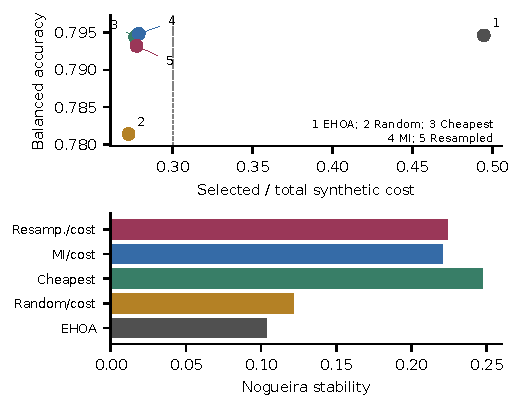
\includegraphics[width=\linewidth]{figures/eligible_comparison.pdf}\par{\footnotesize شکل ۱. میانگین ده دیتاست اجرای تازه؛ هزینه مصنوعی و پایداری توصیفی زیرمجموعه.\par}\end{minipage}\par
\sect{۸  مطالعه پزشکی و ارتباط با کنگره}
داده تشخیصی سرطان پستان شامل ۵۶۹ نمونه آسپیراسیون سوزن ظریف، ۲۱۲ بدخیم و ۳۵۷ خوش‌خیم، با ۳۰ توصیفگر تصویر هسته است \lr{[15].} جدول ۸ و شکل ۲، پانزده ماسک هر روش را نشان می‌دهند. شمارش، انتخاب محاسباتی را توصیف می‌کند، نه زیست‌نشانگر علّی. چند توصیفگر از یک کسب تصویر مشترک می‌آیند؛ هزینه مصنوعی جمع‌پذیر، صرفه‌جویی در قیمت نمونه‌برداری نیست. برچسب \lr{0} بدخیم و \lr{1} خوش‌خیم است؛ بازخوانی هر کلاس صریح گزارش شد.

\par\vspace{3pt}\begin{minipage}{\linewidth}{\footnotesize جدول ۸. سرطان پستان: پانزده اجرا هر روش.\par}
\begin{latin}
{\fontsize{6.8}{8.3}\selectfont\setlength{\tabcolsep}{2pt}\renewcommand{\arraystretch}{1.1}
\begin{tabularx}{\linewidth}{>{\hsize=1.0000\hsize\raggedright\arraybackslash}X>{\hsize=1.0000\hsize\raggedright\arraybackslash}X>{\hsize=1.0000\hsize\raggedright\arraybackslash}X>{\hsize=1.0000\hsize\raggedright\arraybackslash}X>{\hsize=1.0000\hsize\raggedright\arraybackslash}X>{\hsize=1.0000\hsize\raggedright\arraybackslash}X}\toprule
Method & BA & Mal. sens. & Ben. spec. & Cost & Stability\\\midrule
EHOA & 0.9512 & 0.9415 & 0.9608 & 0.5620 & 0.0727\\
Random/cost & 0.9382 & 0.9217 & 0.9546 & 0.2525 & 0.0988\\
Cheapest & 0.9519 & 0.9368 & 0.9669 & 0.2707 & 0.1975\\
MI/cost & 0.9517 & 0.9387 & 0.9647 & 0.2771 & 0.2046\\
Resamp./cost & 0.9493 & 0.9340 & 0.9647 & 0.2751 & 0.1757\\
\bottomrule\end{tabularx}}
\end{latin}
\end{minipage}\par\vspace{3pt}
\par\begin{minipage}{\linewidth}\centering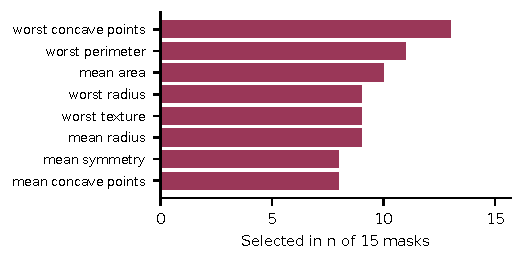
\includegraphics[width=\linewidth]{figures/breast_top_frequencies.pdf}\par{\footnotesize شکل ۲. شمار انتخاب هشت ویژگی پرتکرار در پانزده ماسک تعمیر بازنمونه‌گیری‌شده.\par}\end{minipage}\par
سناریوی خدمت مشترک از تعرفه منتشرشده \lr{Montana} برای تفسیر \lr{FNA} ، کد \lr{88173} ، هزینه \lr{global} برابر \lr{164.34} دلار و تاریخ اثر \lr{2024-06-30} استفاده می‌کند \lr{[17].} هر۳۰ستون \lr{WDBC} از تصویر \lr{FNA} مشتق‌اند \lr{[15]}؛ نگاشت به یک گروه کسب، فرض سناریو است نه فاکتور تأییدشده. هر۷۵ماسک اصلی ناتهی سرطان پستان کل تعرفه مشترک را حفظ می‌کند: صرفه‌جویی خدمت صفر و زیرمجموعه ناتهی در بودجه گروهی۳۰٪ ناممکن است. هزینه جمع‌آوری، زمان محاسبه، خطر و هزینه حاشیه‌ای نامعلوم‌اند.

پروتکل انتقال\lr{7f716c5} پیش از۲۵ برازش فقط روی \lr{Oxford195} ثبت عمومی شد؛ تقسیم درونی گروهی است. مقصد \lr{UCI489}،۲۴۰ ضبط/۸۰ فرد (۴۰بیمار/۴۰کنترل) دارد \lr{[16].} فقط \lr{RPDE/DFA/PPE} مشترک‌اند؛ هزینه مصنوعی برابر، یک ویژگی برای تعمیر مجاز می‌کند. احتمال پنج بذر، سپس سه ضبط هر فرد با آستانه\lr{0.5} تجمیع می‌شود. برچسب مقصد فقط ارزیابی است. فاصله \lr{bootstrap} طبقه‌بندی‌شده۱۰۰۰۰تکراری فردی، توصیفی و شرطی به مدل است و عدم‌قطعیت آموزش را پوشش نمی‌دهد.

\par\vspace{3pt}\begin{minipage}{\linewidth}{\footnotesize جدول۹. انتقال سه‌ویژگی بیرونی؛ \lr{ensemble} فردمحور پنج‌بذری. \lr{E=EHOA} ؛ \lr{R/C/M/S} تعمیرها. فاصله \lr{BA} شامل \lr{0.5} است؛ برتری بالینی نداریم.\par}
\begin{latin}
{\fontsize{6.8}{8.3}\selectfont\setlength{\tabcolsep}{2pt}\renewcommand{\arraystretch}{1.1}
\begin{tabularx}{\linewidth}{>{\hsize=1.0000\hsize\raggedright\arraybackslash}X>{\hsize=1.0000\hsize\raggedright\arraybackslash}X>{\hsize=1.0000\hsize\raggedright\arraybackslash}X>{\hsize=1.0000\hsize\raggedright\arraybackslash}X}\toprule
Methods & BA [95\% descriptive] & Sens./Spec. & AUC\\\midrule
E & 0.575 [0.475,0.675] & 0.725/0.425 & 0.5794\\
R/C/M/S & 0.575 [0.475,0.675] & 0.725/0.425 & 0.5500\\
\bottomrule\end{tabularx}}
\end{latin}
\end{minipage}\par\vspace{3pt}
\sect{۹  محدودیت‌ها و بازتولیدپذیری}
جست‌وجوی متناهی همگرایی را ثابت نمی‌کند؛ فاکتوریل و جست‌وجوی بزرگ‌تر یک بذر دارند. \lr{MI} حاشیه‌ای منهای \lr{SD} تضمین پوشش کالیبره یا کنترل انتخاب کاذب ندارد. زمان‌ها سه/شش پردازش دارند. هویت ضبط اولیه و سوابق تاریخی مفقود تأیید نشده‌اند. انتقال سه‌ویژگی از نام مشترک استفاده می‌کند، بدون تأیید معادل‌بودن استخراج/کالیبراسیون؛ مدل اصلی۲۲ویژگی یا کاربرد آینده‌نگر بالینی را اعتبارسنجی نمی‌کند.

مخزن \lr{github.com/Amirgh23/coststable-ehoa} کد، داده و ممیزی را دارد. بازبرازش۱۴۶۴ طبقه‌بند نهایی و۲۵ انتقال اختلاف پیش‌بینی نداشت؛۷۵ بازاجرای منتخب ماسک تاریخی را بازتولید کردند. این بررسی محیط فعلی است، نه بازیابی لاگ تاریخی یا بازاجرای تمام جست‌وجوها.

\sect{۱۰  نتیجه‌گیری}
تعمیر محلی بودجه مصنوعی را رعایت می‌کند. فیلترهای بدون جست‌وجو پایداری توصیفی بسیار بیشتری دارند؛ برتری پیش‌بینی و ضرورت \lr{EHOA} ثابت نشده است. نتیجه شرطی به یک بردار هزینه مصنوعی برای هر بُعد و پایپ‌لاین \lr{KNN/SMOTE} است. اعتبارسنجی کامل بالینی و هزینه حاشیه‌ای اندازه‌گیری‌شده موجود نیست.

\sect{مراجع}
\begin{minipage}{\linewidth}{\fontsize{7}{8.2}\selectfont \begin{latin}[1] R. Jagdhuber, M. Lang, A. Stenzl, J. Neuhaus, and J. Rahnenführer, "Cost-Constrained feature selection in binary classification: adaptations for greedy forward selection and genetic algorithms," BMC Bioinformatics, vol. 21, art. 26, 2020. \url{https://doi.org/10.1186/s12859-020-3361-9}\end{latin}\par}\end{minipage}\par
\begin{minipage}{\linewidth}{\fontsize{7}{8.2}\selectfont \begin{latin}[2] S. Nogueira, K. Sechidis, and G. Brown, "On the Stability of Feature Selection Algorithms," Journal of Machine Learning Research, vol. 18, no. 174, pp. 1-54, 2018. \url{https://jmlr.org/papers/v18/17-514.html}\end{latin}\par}\end{minipage}\par
\begin{minipage}{\linewidth}{\fontsize{7}{8.2}\selectfont \begin{latin}[3] B. Remeseiro and V. Bolon-Canedo, "A review of feature selection methods in medical applications," Computers in Biology and Medicine, vol. 112, art. 103375, 2019. \url{https://doi.org/10.1016/j.compbiomed.2019.103375}\end{latin}\par}\end{minipage}\par
\begin{minipage}{\linewidth}{\fontsize{7}{8.2}\selectfont \begin{latin}[4] A. E. Hegazy, M. A. Makhlouf, O. A. M. Salem, and B. Hafiz, "An enhanced Hiking optimization algorithm for accurate and interpretable feature selection in medical data classification," Cluster Computing, vol. 29, art. 244, 2026. \url{https://doi.org/10.1007/s10586-026-05946-9}\end{latin}\par}\end{minipage}\par
\begin{minipage}{\linewidth}{\fontsize{7}{8.2}\selectfont \begin{latin}[5] V. Hamer and P. Dupont, "An Importance Weighted Feature Selection Stability Measure," Journal of Machine Learning Research, vol. 22, no. 116, pp. 1-57, 2021. \url{https://jmlr.org/papers/v22/20-366.html}\end{latin}\par}\end{minipage}\par
\begin{minipage}{\linewidth}{\fontsize{7}{8.2}\selectfont \begin{latin}[6] T. Klonecki and P. Teisseyre, "Feature selection under budget constraint in medical applications: analysis of penalized empirical risk minimization methods," Applied Intelligence, vol. 53, pp. 29943-29973, 2023. \url{https://doi.org/10.1007/s10489-023-05063-9}\end{latin}\par}\end{minipage}\par
\begin{minipage}{\linewidth}{\fontsize{7}{8.2}\selectfont \begin{latin}[7] M. Valancius, M. Lennon, and J. Oliva, "Acquisition Conditioned Oracle for Nongreedy Active Feature Acquisition," Proceedings of the 41st International Conference on Machine Learning, PMLR, vol. 235, pp. 48957-48975, 2024. \url{https://proceedings.mlr.press/v235/valancius24a.html}\end{latin}\par}\end{minipage}\par
\begin{minipage}{\linewidth}{\fontsize{7}{8.2}\selectfont \begin{latin}[8] T. Klonecki, P. Teisseyre, and J. Lee, "Cost-Constrained Multi-label Group Feature Selection Using Shadow Features," in Advances in Artificial Intelligence Research, PP-RAI 2025, Lecture Notes in Networks and Systems, vol. 1599, pp. 3-16, Springer, 2026. \url{https://doi.org/10.1007/978-3-032-04197-5_1}\end{latin}\par}\end{minipage}\par
\begin{minipage}{\linewidth}{\fontsize{7}{8.2}\selectfont \begin{latin}[9] N. Meinshausen and P. Buhlmann, "Stability selection," Journal of the Royal Statistical Society: Series B, vol. 72, no. 4, pp. 417-473, 2010. \url{https://doi.org/10.1111/j.1467-9868.2010.00740.x}\end{latin}\par}\end{minipage}\par
\begin{minipage}{\linewidth}{\fontsize{7}{8.2}\selectfont \begin{latin}[10] R. D. Shah and R. J. Samworth, "Variable selection with error control: another look at stability selection," Journal of the Royal Statistical Society: Series B, vol. 75, no. 1, pp. 55-80, 2013. \url{https://doi.org/10.1111/j.1467-9868.2011.01034.x}\end{latin}\par}\end{minipage}\par
\begin{minipage}{\linewidth}{\fontsize{7}{8.2}\selectfont \begin{latin}[11] B. C. Ross, "Mutual Information between Discrete and Continuous Data Sets," PLOS ONE, vol. 9, no. 2, art. e87357, 2014. \url{https://doi.org/10.1371/journal.pone.0087357}\end{latin}\par}\end{minipage}\par
\begin{minipage}{\linewidth}{\fontsize{7}{8.2}\selectfont \begin{latin}[12] N. V. Chawla, K. W. Bowyer, L. O. Hall, and W. P. Kegelmeyer, "SMOTE: Synthetic Minority Over-sampling Technique," Journal of Artificial Intelligence Research, vol. 16, pp. 321-357, 2002. \url{https://doi.org/10.1613/jair.953}\end{latin}\par}\end{minipage}\par
\begin{minipage}{\linewidth}{\fontsize{7}{8.2}\selectfont \begin{latin}[13] S. Varma and R. Simon, "Bias in error estimation when using cross-validation for model selection," BMC Bioinformatics, vol. 7, art. 91, 2006. \url{https://doi.org/10.1186/1471-2105-7-91}\end{latin}\par}\end{minipage}\par
\begin{minipage}{\linewidth}{\fontsize{7}{8.2}\selectfont \begin{latin}[14] J. Demšar, "Statistical Comparisons of Classifiers over Multiple Data Sets," Journal of Machine Learning Research, vol. 7, pp. 1-30, 2006. \url{https://jmlr.org/papers/v7/demsar06a.html}\end{latin}\par}\end{minipage}\par
\begin{minipage}{\linewidth}{\fontsize{7}{8.2}\selectfont \begin{latin}[15] W. Wolberg, O. Mangasarian, N. Street, and W. Street, "Breast Cancer Wisconsin (Diagnostic)," UCI Machine Learning Repository, 1993. \url{https://doi.org/10.24432/C5DW2B}\end{latin}\par}\end{minipage}\par
\begin{minipage}{\linewidth}{\fontsize{7}{8.2}\selectfont \begin{latin}[16] C. Prez, "Parkinson Dataset with replicated acoustic features," UCI, 2016. \url{https://doi.org/10.24432/C5701F}\end{latin}\par}\end{minipage}\par
\begin{minipage}{\linewidth}{\fontsize{7}{8.2}\selectfont \begin{latin}[17] Montana DPHHS, "Cancer Control Programs Fee for Service Schedule," effective June 30, 2024,p.3,code 88173. \url{https://dphhs.mt.gov/assets/publichealth/Cancer/MCCP2025FeeSchedule.pdf}\end{latin}\par}\end{minipage}\par
\begin{minipage}{\linewidth}{\fontsize{7}{8.2}\selectfont \begin{latin}[18] R. Jagdhuber and J. Rahnenführer, "Implications on Feature Detection when using the Benefit-Cost Ratio," arXiv:2008.05163v2, 2020. \url{https://doi.org/10.48550/arXiv.2008.05163}\end{latin}\par}\end{minipage}\par
\end{multicols}
\end{document}